% !TEX program = xelatex
\documentclass[12pt,a4paper]{article}
\usepackage{geometry}
\geometry{top=0.8cm, bottom=0.5cm, left=0.8cm, right=0.8cm}
\usepackage{fontspec}
\setmainfont{TH Sarabun New}[Scale=1.4]
\usepackage{tikz}
\usepackage{multirow}
\usepackage{array}
\usepackage{hhline}

% --- MC bubble with label inside ---
\newcommand{\mcbubble}[2]{%
  \begin{tikzpicture}[scale=1.0]
    \draw[thick] (0,0) circle (3.8pt);
    \node at (0,0.02) {\fontsize{6.5pt}{7pt}\selectfont #1};
  \end{tikzpicture}%
}

% --- MC question: number + 4 inline bubbles ---
\newcommand{\mcquestion}[1]{%
  \fontsize{8pt}{9pt}\selectfont #1.\hspace{1pt}%
  \mcbubble{ก}{}\hspace{1pt}%
  \mcbubble{ข}{}\hspace{1pt}%
  \mcbubble{ค}{}\hspace{1pt}%
  \mcbubble{ง}{}%
}

% --- digit column (0-9) ---
\newcommand{\digitcol}[1]{%
  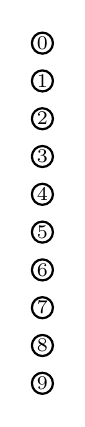
\begin{tikzpicture}[scale=1.0]
    \foreach \y/\n in {0/9, 0.48/8, 0.96/7, 1.44/6, 1.92/5, 2.40/4, 2.88/3, 3.36/2, 3.84/1, 4.32/0} {
      \draw[thick] (0,\y) circle (3.8pt);
      \node at (0,\y) {\fontsize{7pt}{8pt}\selectfont \n};
    }
  \end{tikzpicture}%
}

% --- fill-in question: 4-column table ---
\newcommand{\fillinquestion}[2]{%
  \fontsize{10pt}{12pt}\selectfont \textbf{ข้อ #1} \\[0.5mm]
  \begin{tabular}{|c|c|c|c|}
  \hline
  \multicolumn{1}{|c|}{\fontsize{8pt}{9pt}\selectfont หลักพัน} &
  \multicolumn{1}{c|}{\fontsize{8pt}{9pt}\selectfont หลักร้อย} &
  \multicolumn{1}{c|}{\fontsize{8pt}{9pt}\selectfont หลักสิบ} &
  \multicolumn{1}{c|}{\fontsize{8pt}{9pt}\selectfont หลักหน่วย} \\
  \hline
  \digitcol{0} & \digitcol{1} & \digitcol{2} & \digitcol{3} \\
  \hline
  \end{tabular}%
}

\begin{document}
\pagestyle{empty}

% --- title ---
\begin{center}
{\fontsize{16pt}{18pt}\selectfont \textbf{กระดาษคำตอบ}}
\end{center}
\vspace{1mm}

% --- student info ---
\noindent
{\fontsize{10pt}{12pt}\selectfont
\textbf{ชื่อ-นามสกุล} \dotfill \hspace{1cm}
\textbf{ชั้น} \dotfill \hspace{1cm}
\textbf{ชื่อเล่น} \dotfill
}
\vspace{1mm}

% --- multiple choice section ---
\noindent
{\fontsize{11pt}{13pt}\selectfont \textbf{ตอนที่ 1--2 ปรนัย (ข้อ 1--55)}} \hfill
{\fontsize{8pt}{9pt}\selectfont \textbf{คำเตือน:} ระบายตัวเลือก \textbf{เพียงข้อเดียว} ในแต่ละข้อ ถ้าต้องการเปลี่ยนคำตอบ ให้ลบข้อเดิมออกก่อน}

\vspace{2mm}


\noindent
{\fontsize{10pt}{12pt}\selectfont \textbf{คณิตศาสตร์ (ข้อ 1–30)}}
\vspace{1mm}

\noindent
\begin{tabular}{p{0.18\textwidth}p{0.18\textwidth}p{0.18\textwidth}p{0.18\textwidth}p{0.18\textwidth}}
\mcquestion{1} & \mcquestion{7} & \mcquestion{13} & \mcquestion{19} & \mcquestion{25} \\[1pt]
\mcquestion{2} & \mcquestion{8} & \mcquestion{14} & \mcquestion{20} & \mcquestion{26} \\[1pt]
\mcquestion{3} & \mcquestion{9} & \mcquestion{15} & \mcquestion{21} & \mcquestion{27} \\[1pt]
\mcquestion{4} & \mcquestion{10} & \mcquestion{16} & \mcquestion{22} & \mcquestion{28} \\[1pt]
\mcquestion{5} & \mcquestion{11} & \mcquestion{17} & \mcquestion{23} & \mcquestion{29} \\[1pt]
\mcquestion{6} & \mcquestion{12} & \mcquestion{18} & \mcquestion{24} & \mcquestion{30} \\[1pt]
\end{tabular}
\vspace{2mm}

\noindent
{\fontsize{10pt}{12pt}\selectfont \textbf{วิทยาการคำนวณ (ข้อ 31–55)}}
\vspace{1mm}

\noindent
\begin{tabular}{p{0.18\textwidth}p{0.18\textwidth}p{0.18\textwidth}p{0.18\textwidth}p{0.18\textwidth}}
\mcquestion{31} & \mcquestion{36} & \mcquestion{41} & \mcquestion{46} & \mcquestion{51} \\[1pt]
\mcquestion{32} & \mcquestion{37} & \mcquestion{42} & \mcquestion{47} & \mcquestion{52} \\[1pt]
\mcquestion{33} & \mcquestion{38} & \mcquestion{43} & \mcquestion{48} & \mcquestion{53} \\[1pt]
\mcquestion{34} & \mcquestion{39} & \mcquestion{44} & \mcquestion{49} & \mcquestion{54} \\[1pt]
\mcquestion{35} & \mcquestion{40} & \mcquestion{45} & \mcquestion{50} & \mcquestion{55} \\[1pt]
\end{tabular}

\vspace{2mm}
\noindent
{\fontsize{11pt}{13pt}\selectfont \textbf{ตอนที่ 3 อัตนัย เติมคำตอบ (ข้อ 56--60)}}
\vspace{2mm}

\noindent
{\fontsize{8pt}{9pt}\selectfont \textbf{วิธีระบาย:} แต่ละข้อมี 4 หลัก (พัน ร้อย สิบ หน่วย) ให้ระบายตัวเลข\textbf{หนึ่งตัวต่อหนึ่งหลัก} หากคำตอบมีค่าน้อยกว่า 4 หลัก ให้ระบาย \textbf{0} นำหน้าในหลักที่สูงกว่า (เช่น ตอบ 42 ให้ระบาย หลักพัน=0, หลักร้อย=0, หลักสิบ=4, หลักหน่วย=2)}
\vspace{3mm}

\noindent\centering
\begin{minipage}[t]{0.32\textwidth}\centering
\fillinquestion{56}{4}
\end{minipage}
\begin{minipage}[t]{0.32\textwidth}\centering
\fillinquestion{57}{4}
\end{minipage}
\begin{minipage}[t]{0.32\textwidth}\centering
\fillinquestion{58}{4}
\end{minipage}
\\[2mm]
\begin{minipage}[t]{0.32\textwidth}\centering
\fillinquestion{59}{4}
\end{minipage}
\begin{minipage}[t]{0.32\textwidth}\centering
\fillinquestion{60}{4}
\end{minipage}
\\[2mm]
\vfill
\begin{center}
{\fontsize{8pt}{9pt}\selectfont จัดทำโดย พี่หยวน}
\end{center}
\end{document}
